\documentclass[10pt]{beamer}

\usepackage[ruled,vlined,english]{algorithm2e}
\DontPrintSemicolon

\usepackage{graphicx}
\usepackage[normalem]{ulem}
\usepackage{color,soul}
\usepackage{multirow}
\usepackage{tikz}
\usetikzlibrary{decorations.pathreplacing}
\usetikzlibrary{calc}
\usetikzlibrary{positioning}
\usetikzlibrary{arrows.meta}
\usetikzlibrary{shapes}
\usetheme[numbering=fraction,titleformat=smallcaps,progressbar=frametitle]{metropolis}
\usepackage[normalem]{ulem}

\usepackage{svg}

\usepackage[binary-units,group-digits,group-separator={,}]{siunitx}
\DeclareSIUnit\flop{Flop}
\DeclareSIUnit\flops{\flop\per\second}
\newcommand{\Num}[1]{\num[group-separator={,}]{#1}\xspace}
\newcommand{\NSI}[2]{\SI[group-separator={,}]{#1}{#2}\xspace}


% From https://github.com/matze/mtheme/issues/237#issuecomment-258718692
\makeatletter
\setlength{\metropolis@titleseparator@linewidth}{1.5pt}
\setlength{\metropolis@progressonsectionpage@linewidth}{1.5pt}
\setlength{\metropolis@progressinheadfoot@linewidth}{1pt}
\makeatother

\usepackage{fontawesome}

\newcommand{\backupbegin}{
   \newcounter{framenumberappendix}
   \setcounter{framenumberappendix}{\value{framenumber}}
}
\newcommand{\backupend}{
   \addtocounter{framenumberappendix}{-\value{framenumber}}
   \addtocounter{framenumber}{\value{framenumberappendix}}
}

% Command to make the last slide, which shows copies of the other slides
\newcommand{\addframe}[1] {\includegraphics[page=#1, width=0.3\textwidth]{demo_old.pdf}}

% *** SPECIFIC MACROS ***
% specific macro definition for the paper
%
% requires amsthm, xspace

% theorem-like environment
\newtheorem{thm}{Theorem}
\newtheorem{lem}[thm]{Lemma}
\newtheorem{prop}{Proposition}
\newtheorem{propty}{Property}
\newtheorem{defn}{Definition}

% asymptotic complexity (Landau) notations
\newcommand{\landauO}{\ensuremath{\mathcal{O}}\xspace}
\newcommand{\landauOmega}{\ensuremath{\Omega}\xspace}
\newcommand{\landauTheta}{\ensuremath{\Theta}\xspace}
\newcommand{\landauo}{\ensuremath{o}\xspace}
\newcommand{\landauomega}{\ensuremath{\omega}\xspace}
\newcommand{\landauorder}{\ensuremath{\sim}\xspace}

% scheduling notations
\newcommand{\graham}[3]{\mbox{\ensuremath{#1\mid#2\mid#3}}}
\newcommand{\Cmax}{\ensuremath{C_{\max}}\xspace}

% complexity classes
\newcommand{\cNP}{\textbf{NP}\xspace}  % bold notations
\newcommand{\cP}{\textbf{P}\xspace}
% \newcommand{\cNP}{\ensuremath{\mathcal{N\!P}}\xspace}  % round notations
% \newcommand{\cP}{\ensuremath{\mathcal{P}}\xspace}

% Machine states
\newcommand{\computing}{computing}
\newcommand{\idle}{idle}
\newcommand{\off}{of\!f}
\newcommand{\on}{on}
\newcommand{\ontooff}{\on\rightarrow\off}
\newcommand{\offtoon}{\off\rightarrow\on}

% CCGRID 2017
\newcommand{\ra}[1]{\renewcommand{\arraystretch}{#1}}

% Cluster 2017
\newcommand{\overbar}[1]{\mkern 1.5mu\overline{\mkern-1.5mu#1\mkern-1.5mu}\mkern 1.5mu}

\newlength\mylen % algorithm2e hack
\newcommand\myinput[1]{%
  \settowidth\mylen{\KwIn{}}%
  \setlength\hangindent{\mylen}%
  \hspace*{\mylen}#1\\}

\newcommand\myoutput[1]{% algorithm2e hack
  \settowidth\mylen{\KwOut{}}%
  \setlength\hangindent{\mylen}%
  \hspace*{\mylen}#1\\}



%%%%%%%%%%%%%%%%%%%%%%%
% Modular compilation %
%%%%%%%%%%%%%%%%%%%%%%%
\newif\ifwatermark
\watermarktrue

\newif\iftotalcompilation
\totalcompilationtrue

\newcommand{\inputchapter}[2]{%
  \ifdef{#1}%
    {\input{#2}\cleardoublepage}%
    {}%
}

% Modeling notations
\newcommand{\model}[2][]{\ensuremath{\bm{M}_{#1}\ifthenelse{\equal{#2}{}}{}{\!-\!}{#2}}\xspace}
\newcommand{\modelp}[2][]{\ensuremath{\bm{M'}_{#1}\!\ifthenelse{\equal{#2}{}}{}{\!-\!}{#2}}\xspace}
\newcommand{\noise}[2][]{\ensuremath{\bm{N}_{#1}\ifthenelse{\equal{#2}{}}{}{\!-\!}{#2}}\xspace}
\newcommand{\noisep}[2][]{\ensuremath{\bm{N'}_{#1}\!\ifthenelse{\equal{#2}{}}{}{\!-\!}{#2}}\xspace}
\newcommand{\norm}{\ensuremath{\mathcal{N}}\xspace}
\newcommand{\mcdots}{\ensuremath{\!\cdot\!\cdot\!\cdot\!}\xspace}
\newcommand{\unif}[2]{\ensuremath{\mathcal{U}\left({#1},{#2}\right)}\xspace}

% Abreviations
\newcommand{\eg}{e.g.\@\xspace}
\newcommand{\ie}{i.e.\@\xspace}
\newcommand{\aka}{a.k.a.\@\xspace}
\newcommand{\resp}{resp.\@\xspace}
\newcommand{\etal}{et~al.\@\xspace}
\newcommand{\dgemm}{\texttt{dgemm}\@\xspace}
\newcommand{\recv}{\texttt{MPI\_Recv}\@\xspace}
\newcommand{\send}{\texttt{MPI\_Send}\@\xspace}
\newcommand{\isend}{\texttt{MPI\_Isend}\@\xspace}
\newcommand{\iprobe}{\texttt{MPI\_Iprobe}\@\xspace}
\newcommand{\pyce}{\texttt{pycewise}\@\xspace}

% Referencing several times a footnote
% See https://tex.stackexchange.com/a/54240
\newcommand{\savefootnote}[2]{\footnote{\label{#1}#2}}
\newcommand{\repeatfootnote}[1]{\textsuperscript{\ref{#1}}}


\definecolor{darkgray}{HTML}{333333}
\definecolor{gray}{HTML}{4D4D4D}
\definecolor{lightgray}{HTML}{BBBBBB}
\definecolor{green}{HTML}{C2E15F}
\definecolor{orange}{HTML}{FDA333}
\definecolor{purple}{HTML}{D3A4F9}
\definecolor{red}{HTML}{FB4485}
\definecolor{blue}{HTML}{6CE0F1}
\definecolor{pblue}{HTML}{0395DE}
\definecolor{materialpurple}{HTML}{9C27B0}
\definecolor{materialindigo}{HTML}{3F51B5}
\definecolor{materialblue}{HTML}{2196F3}
\definecolor{materialcyan}{HTML}{00BCD4}
\definecolor{materialteal}{HTML}{009688}
\definecolor{materialgreen}{HTML}{4CAF50}
\definecolor{materiallime}{HTML}{CDDC39}
\definecolor{materialamber}{HTML}{FFC107}
\definecolor{materialbrown}{HTML}{795548}
\definecolor{materialred}{HTML}{FF4436}
\definecolor{materialorange}{HTML}{FF5722}
\setbeamercolor{normal text}{bg=white}
\colorlet{mycolor}{materialblue}
\setbeamercolor{alerted text}{fg=mycolor}

% Yes, we really need this kind of crap to remove the space before the itemize, WTF Latex ?!
% Relevant links:
%  - https://tex.stackexchange.com/questions/86054/how-to-remove-the-whitespace-before-itemize-enumerate
%  - https://tex.stackexchange.com/questions/24371/does-enumitem-conflict-with-beamer-for-lists
\usepackage{enumitem}
\setitemize{label=\usebeamerfont*{itemize item}%
  \usebeamercolor[fg]{itemize item}
  \usebeamertemplate{itemize item}}
%\setlist[itemize]{noitemsep, topsep=0pt}

\renewcommand{\emph}[1]{\SoulColor{lightorange}\hl{#1}}
\makeatletter
\let\HL\hl
\renewcommand\hl{%
  \let\set@color\beamerorig@set@color
  \let\reset@color\beamerorig@reset@color
  \HL}
\colorlet{mycolorlight}{mycolor!30}
\sethlcolor{mycolorlight}
\makeatother
\renewcommand<>{\hl}[1]{\only#2{\beameroriginal{\hl}}{#1}}
\renewcommand<>{\emph}[1]{\only#2{\beameroriginal{\hl}}{#1}}


\setlength{\interspacetitleruled}{0pt}%
\setlength{\algotitleheightrule}{0pt}%

% Using a small font for verbatim blocks
\def\changefont#1{%
  \setbeamertemplate{itemize/enumerate body begin}{#1}
  \setbeamertemplate{itemize/enumerate subbody begin}{#1}
  #1}
\makeatletter
\newcommand{\verbatimfont}[1]{\renewcommand{\verbatim@font}{\ttfamily#1}}
\makeatother
\verbatimfont{\scriptsize}%small
\let\endmintedbak=\endminted
\def\endminted{\endmintedbak\vspace{-1cm}}


\date{}
\author{Tom Cornebize}
\date{2 June 2021, PhD defense}
\title{High Performance Computing: Towards Better Performance Predictions and Experiments}

\begin{document}
\titlegraphic{
    \begin{picture}(0,0)
        \put(310,-200){\makebox(0,0)[rt]{
            \begin{minipage}{\textwidth}
                \includesvg[height=1cm]{img/logo_uga.svg}\hfill%
                
\includegraphics[height=1cm]{img/logo_cnrs.png}\hfill%
                
\includegraphics[height=1cm]{img/logo_inria.png}
            \end{minipage}
        }}
    \end{picture}
}

\maketitle

\begin{frame}{No science without computing}
    \begin{columns}
        \begin{column}[c]{.33\columnwidth}
            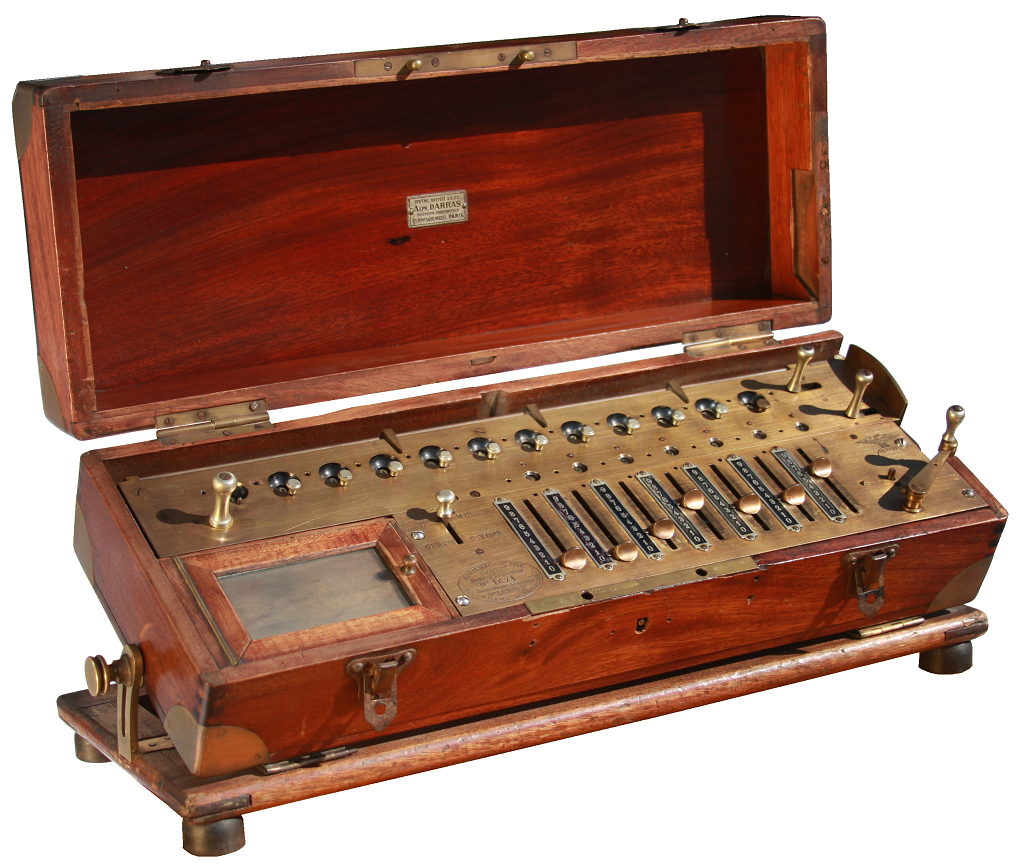
\includegraphics[width=\linewidth]{img/arithmometer.png}
            Arithmometer (1851)
        \end{column}
        \begin{column}[c]{.33\columnwidth}
            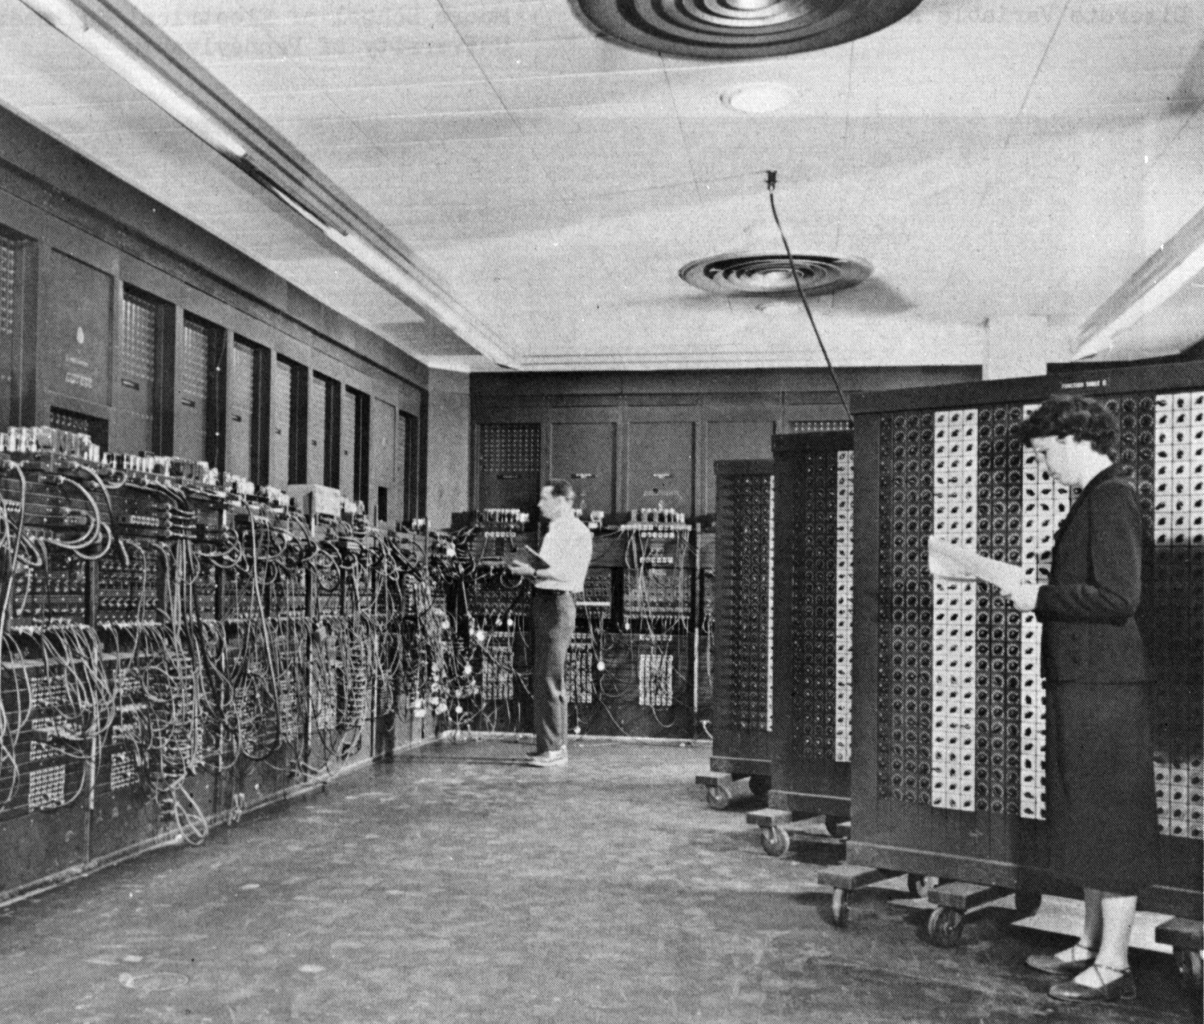
\includegraphics[width=\linewidth]{img/eniac.jpg}
            ENIAC (1945)
        \end{column}
        \begin{column}[c]{.33\columnwidth}
            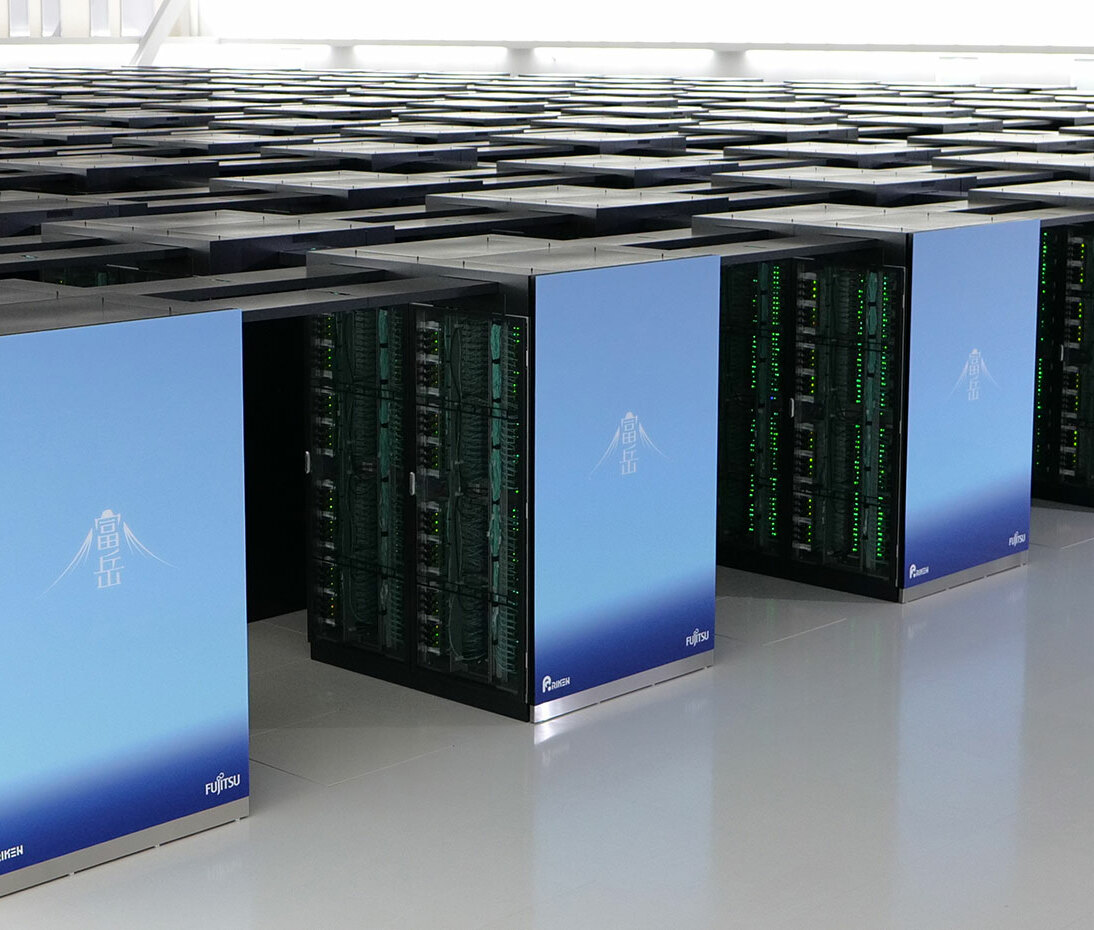
\includegraphics[width=\linewidth]{img/fugaku.jpg}
            Fugaku (2021)
        \end{column}
    \end{columns}
    \vfill

    \pause

    Last decades:
    \begin{itemize}
        \item Exponential \alert{performance} improvements
        (\eg sequencing an entire human genome costed \SI{100000000}[\$]{} in 2001, \SI{1000}[\$]{} now)
        \item At the price of \alert{complexity} (both software and hardware)
    \end{itemize}
\end{frame}

\begin{frame}{Experimental study of computer performance}
    \begin{columns}
        \begin{column}[c]{.5\columnwidth}
            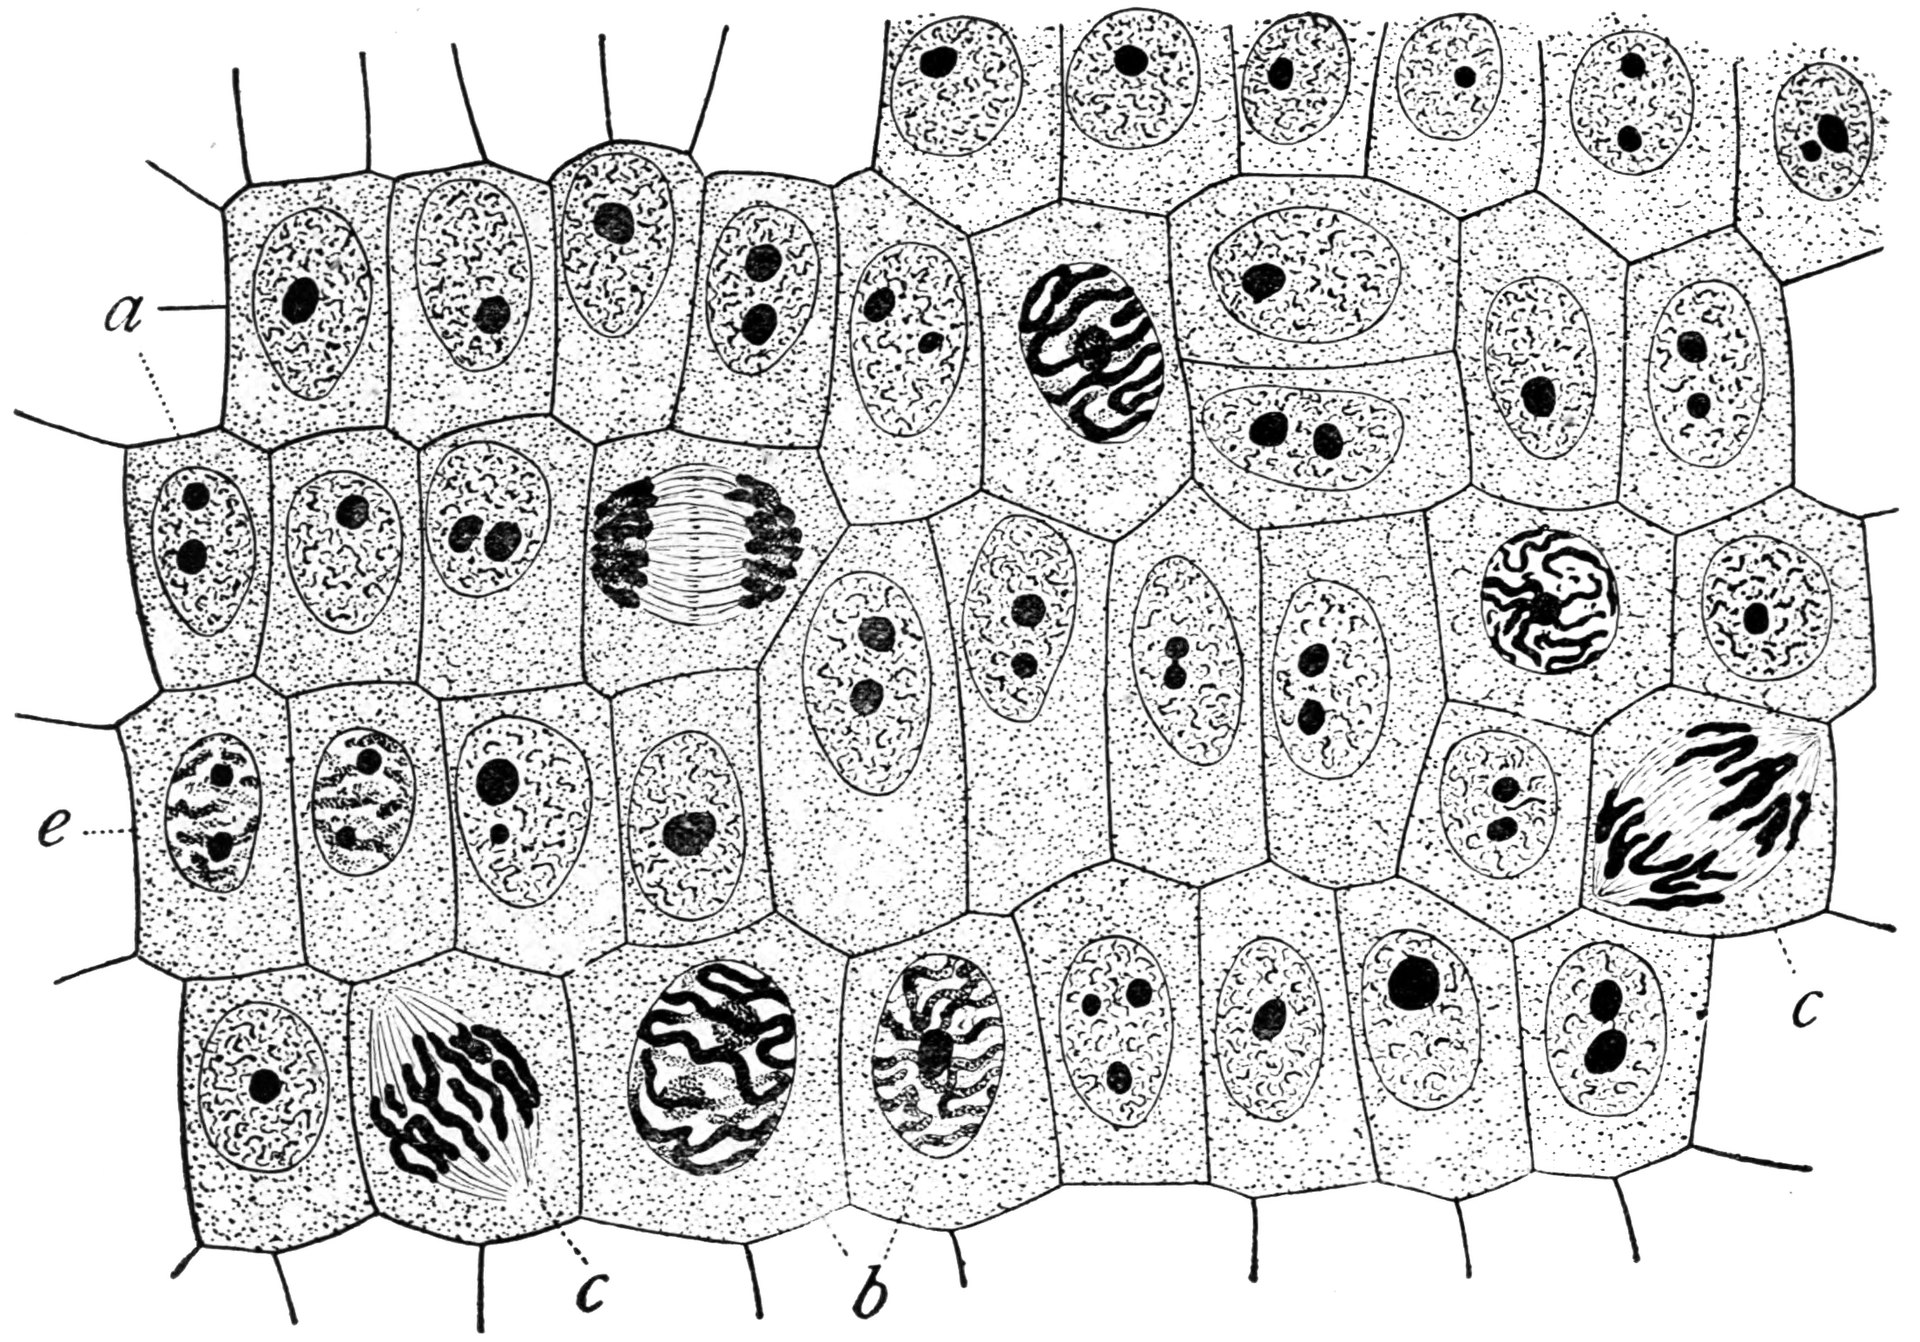
\includegraphics[width=\linewidth]{img/cells.jpg}
        \end{column}
        \begin{column}[c]{.5\columnwidth}
            Similar to natural sciences
            \begin{flalign*}
                \text{Complexity} &\Rightarrow \text{Variability and Opacity}&\\
                                  &\Rightarrow \text{No perfect model}&\\
                                  &\Rightarrow \text{Need for \alert{experiments}}&\\
            \end{flalign*}
        \end{column}
    \end{columns}
    \pause
    \vfill
    Experiments can be carried in \alert{reality} or in \alert{simulation}
\end{frame}

\begin{frame}{Context}
    \textbf{Typical Performance Evaluation Questions} (Given my application and a supercomputer)

    \begin{minipage}[m]{0.35\linewidth}
        
\includegraphics[width=\textwidth]{img/computer_guy_meme.pdf}
    \end{minipage} %
    \begin{minipage}[m]{0.64\linewidth}
    \begin{itemize}
        \item \textbf{Before} running
        \begin{itemize}
            \item How many nodes?
            \item For how long?
            \item Which parameters?
        \end{itemize}
        \pause
        \item \textbf{After} running
        \begin{itemize}
            \item Performance as ``expected''?
            \item Problem in the app or the platform?
        \end{itemize}
    \end{itemize}
    \end{minipage}
    \pause

    \begin{center}
        So many large-scale runs, solely to tune performance?!?
    \end{center}

    \pause

    \textbf{Holy Grail: Predictive Simulation on a ``Laptop''}

    Capture the \textbf{whole application}  and \textbf{platform complexity}
\end{frame}

\begin{frame}[plain]
    \onslide<+->
    \begin{LARGE}
        Initial goal: \alert{\textbf{predict}} the performance of a parallel application
    \end{LARGE}
    \vfill
    \onslide<+->
    \begin{block}{Thesis contributions (towards this goal)}
        \begin{itemize}
            \item Case study: High Performance Linpack (HPL)
            \item Extensive (in)validation, comparing simulations with reality
            \item Modeling correctly the platform variability is key
        \end{itemize}
    \end{block}
    \onslide<+->
    \begin{block}{Thesis contributions (made on the way)}
        \begin{itemize}
            \item \textcolor<+->{lightgray}{Automation (of experiments, statistical analyzes, etc.)}
            \item \textcolor<.>{lightgray}{Experiment methodology, to bias or not to bias}
            \item Performance tests, to detect eventual platform changes
        \end{itemize}
    \end{block}
\end{frame}

\begin{frame}[fragile]{Sim(Em)ulation: The SMPI Approach}
    \begin{columns}
        \begin{column}[c]{.2\columnwidth}
            \scalebox{.8}{\begin{tikzpicture}[xscale=1,yscale=1]
                \node (nodehost) [name=nodehost]
                { 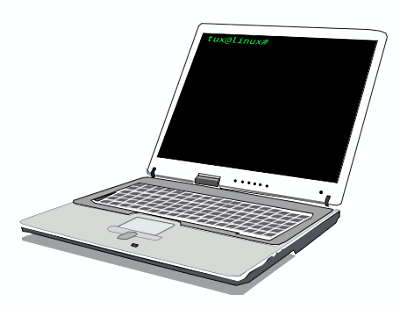
\includegraphics[height=23mm]{img/laptop.png}};

                %\node (nodelisting) [above right= -25mm of nodehost]%, overlay]
                % { \includegraphics[height=12mm]{fig/mpi-codelisting.png}};

                \node (nodeimagine) [
                    shape             = cloud callout,
                    cloud puffs       = 11,
                    aspect            = 1.5,
                    opacity           =.75,
                    draw              = black!90!white, % colour of the border
                    top color         = white,                % | filling of the node
                    bottom color      = black!30!white, % |
                    text              = black!90!white, % colour of the fonts
                    thick,                              % thickness of the border
                    above             = 5mm of nodehost,
                    minimum height    = 25mm,
                    minimum width     = 30mm,
                    callout pointer shorten=7mm,
                    callout absolute pointer={(285:5mm)},%(nodelisting.northwest)},%(285:5.5mm)},
                ]{};

                \node at (nodeimagine) {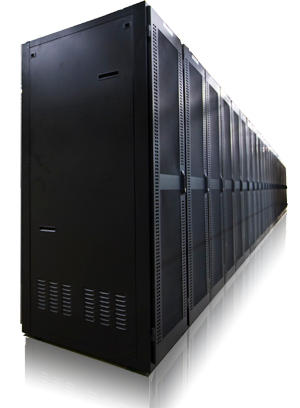
\includegraphics[width=15mm]{img/cluster.png}};
            \end{tikzpicture}}
        \end{column}

        \begin{column}[c]{.85\columnwidth}
            \begin{picture}(0, 0)
                \put(167,-26){\hbox{
                    
\includegraphics[width=2cm]{img/simgrid_logo.pdf}
                }}
            \end{picture}
            \begin{block}{Full reimplementation of MPI on top of}% \alert{SimGrid}}
                \begin{itemize}
                    \item C/C++/F77/F90 codes run \alert{unmodified out of the box}
                    \item Simply replace mpicc/mpirun by smpicc/smpirun
                \end{itemize}
            \end{block}
            \pause
            \begin{block}{Emulation: how?}
                \begin{itemize}
                    \item Computations run for real on a laptop
                    \item Communications are faked, good fluid network models
                    \item \alert{Performance model} for the target platform
                \end{itemize}
            \end{block}
        \end{column}
    \end{columns}
    \pause
    \textbf{Contribution}: Skip the expensive computations (mostly \dgemm) and replace them by performance models
\end{frame}


% See:
%   https://academia.stackexchange.com/a/88068/37904
%   https://unix.stackexchange.com/a/277987/106103
%   https://stackoverflow.com/a/5349842/4110059
%\begin{frame}[plain]
%    \centering
%    \setlength{\tabcolsep}{0pt}
%    \renewcommand{\arraystretch}{0}
%    \begin{tabular}{|c|c|c|}
%        \hline
%        \addframe{1}  & \addframe{6}  & \addframe{9}  \\
%        \hline
%        \addframe{11}  & \addframe{16}  & \addframe{24}  \\
%        \hline
%        \addframe{27}  & \addframe{32}  & \addframe{34}  \\
%        \hline
%        % Some ugly stuff, it would be great to find something better...
%        \vspace{10pt}\\
%        \multicolumn{3}{l}{\alert{\faicon{envelope}} \href{mailto:tom.cornebize@univ-grenoble-alpes.fr}{tom.cornebize@univ-grenoble-alpes.fr}}\\
%    \end{tabular}
%\end{frame}

\end{document}
